%% BioMed_Central_Tex_Template_v1.06
%%                                      %
%  bmc_article.tex            ver: 1.06 %
%                                       %

%%IMPORTANT: do not delete the first line of this template
%%It must be present to enable the BMC Submission system to
%%recognise this template!!

%%%%%%%%%%%%%%%%%%%%%%%%%%%%%%%%%%%%%%%%%
%%                                     %%
%%  LaTeX template for BioMed Central  %%
%%     journal article submissions     %%
%%                                     %%
%%          <8 June 2012>              %%
%%                                     %%
%%                                     %%
%%%%%%%%%%%%%%%%%%%%%%%%%%%%%%%%%%%%%%%%%


%%%%%%%%%%%%%%%%%%%%%%%%%%%%%%%%%%%%%%%%%%%%%%%%%%%%%%%%%%%%%%%%%%%%%
%%                                                                 %%
%% For instructions on how to fill out this Tex template           %%
%% document please refer to Readme.html and the instructions for   %%
%% authors page on the biomed central website                      %%
%% http://www.biomedcentral.com/info/authors/                      %%
%%                                                                 %%
%% Please do not use \input{...} to include other tex files.       %%
%% Submit your LaTeX manuscript as one .tex document.              %%
%%                                                                 %%
%% All additional figures and files should be attached             %%
%% separately and not embedded in the \TeX\ document itself.       %%
%%                                                                 %%
%% BioMed Central currently use the MikTex distribution of         %%
%% TeX for Windows) of TeX and LaTeX.  This is available from      %%
%% http://www.miktex.org                                           %%
%%                                                                 %%
%%%%%%%%%%%%%%%%%%%%%%%%%%%%%%%%%%%%%%%%%%%%%%%%%%%%%%%%%%%%%%%%%%%%%

%%% additional documentclass options:
%  [doublespacing]
%  [linenumbers]   - put the line numbers on margins

%%% loading packages, author definitions

\documentclass[twocolumn]{bmcart}% uncomment this for twocolumn layout and comment line below
%\documentclass{bmcart}

%%% Load packages
\usepackage{amsthm,amsmath}
\usepackage{siunitx}
\usepackage{mfirstuc}
%\RequirePackage{natbib}
\usepackage[colorinlistoftodos]{todonotes}
\RequirePackage{hyperref}
\usepackage[utf8]{inputenc} %unicode support
%\usepackage[applemac]{inputenc} %applemac support if unicode package fails
%\usepackage[latin1]{inputenc} %UNIX support if unicode package fails
\usepackage[htt]{hyphenat}

\usepackage{array}
\newcolumntype{L}[1]{>{\raggedright\let\newline\\\arraybackslash\hspace{0pt}}p{#1}}

%%%%%%%%%%%%%%%%%%%%%%%%%%%%%%%%%%%%%%%%%%%%%%%%%
%%                                             %%
%%  If you wish to display your graphics for   %%
%%  your own use using includegraphic or       %%
%%  includegraphics, then comment out the      %%
%%  following two lines of code.               %%
%%  NB: These line *must* be included when     %%
%%  submitting to BMC.                         %%
%%  All figure files must be submitted as      %%
%%  separate graphics through the BMC          %%
%%  submission process, not included in the    %%
%%  submitted article.                         %%
%%                                             %%
%%%%%%%%%%%%%%%%%%%%%%%%%%%%%%%%%%%%%%%%%%%%%%%%%


%\def\includegraphic{}
%\def\includegraphics{}

%%% Put your definitions there:
\startlocaldefs
\endlocaldefs


%%% Begin ...
\begin{document}

%%% Start of article front matter
\begin{frontmatter}

\begin{fmbox}
\dochead{Report from 2015 Brainhack Americas (MX)}

%%%%%%%%%%%%%%%%%%%%%%%%%%%%%%%%%%%%%%%%%%%%%%
%%                                          %%
%% Enter the title of your article here     %%
%%                                          %%
%%%%%%%%%%%%%%%%%%%%%%%%%%%%%%%%%%%%%%%%%%%%%%

\title{Open source low-cost device to register dog's heart rate and tail
movement}
\vskip2ex
\projectURL{Project URL: \url{https://github.com/nekrum/DogVest}}

\author[
addressref={aff1},
%
email={raul@lafuentelab.org}
]{\inits{RH} \fnm{Raúl} \snm{Hernández-Pérez}}
\author[
addressref={aff1},
%
email={edalvmor@yahoo.com.mx}
]{\inits{EAM} \fnm{Edgar A.} \snm{Morales}}
\author[
addressref={aff1},
corref={aff1},
email={lauveri.rozen@gmail.com}
]{\inits{LVC} \fnm{Laura V.} \snm{Cuaya}}

%%%%%%%%%%%%%%%%%%%%%%%%%%%%%%%%%%%%%%%%%%%%%%
%%                                          %%
%% Enter the authors' addresses here        %%
%%                                          %%
%% Repeat \address commands as much as      %%
%% required.                                %%
%%                                          %%
%%%%%%%%%%%%%%%%%%%%%%%%%%%%%%%%%%%%%%%%%%%%%%

\address[id=aff1]{%
  \orgname{Instituto de Neurobiología},
  \city{Queretaro},
  \street{Boulevard Juriquilla 3001},
  \postcode{76230},
  \postcode{Queretaro},
  \cny{Mexico}
}

%%%%%%%%%%%%%%%%%%%%%%%%%%%%%%%%%%%%%%%%%%%%%%
%%                                          %%
%% Enter short notes here                   %%
%%                                          %%
%% Short notes will be after addresses      %%
%% on first page.                           %%
%%                                          %%
%%%%%%%%%%%%%%%%%%%%%%%%%%%%%%%%%%%%%%%%%%%%%%

\begin{artnotes}
\end{artnotes}

%\end{fmbox}% comment this for two column layout

%%%%%%%%%%%%%%%%%%%%%%%%%%%%%%%%%%%%%%%%%%%%%%
%%                                          %%
%% The Abstract begins here                 %%
%%                                          %%
%% Please refer to the Instructions for     %%
%% authors on http://www.biomedcentral.com  %%
%% and include the section headings         %%
%% accordingly for your article type.       %%
%%                                          %%
%%%%%%%%%%%%%%%%%%%%%%%%%%%%%%%%%%%%%%%%%%%%%%

%\begin{abstractbox}

%\begin{abstract} % abstract
	
%Blank Abstract

%\end{abstract}



%%%%%%%%%%%%%%%%%%%%%%%%%%%%%%%%%%%%%%%%%%%%%%
%%                                          %%
%% The keywords begin here                  %%
%%                                          %%
%% Put each keyword in separate \kwd{}.     %%
%%                                          %%
%%%%%%%%%%%%%%%%%%%%%%%%%%%%%%%%%%%%%%%%%%%%%%

%\vskip1ex

%\projectURL{\url{https://github.com/nekrum/DogVest}}
%\projectURL{https://github.com/nekrum/DogVest}

% MSC classifications codes, if any
%\begin{keyword}[class=AMS]
%\kwd[Primary ]{}
%\kwd{}
%\kwd[; secondary ]{}
%\end{keyword}

%\end{abstractbox}
%
\end{fmbox}% uncomment this for twcolumn layout

\end{frontmatter}

%{\sffamily\bfseries\fontsize{10}{12}\selectfont Project URL: \url{https://github.com/nekrum/DogVest}}

%%% Import the body from pandoc formatted text
\section{Introduction}\label{introduction}

In dogs, the perception of an important stimulus can be related to
physiological changes such as the heart rate (e.g., in socioemotional
situations with humans \cite{Palestrini200575} or dogs
\cite{Siniscalchi20132279} ) and the movement of their tail (e.g.,
tail-wagging has a bias that depends on the nature of the stimulus, a
bias to the left is related to a withdrawal tendency and a bias to the
right is related to an aproach tendency \cite{Quaranta2007R199} ).

Altough heart rate and the tail movement are important gateways to
understand dog's cognition, just a few studies report these variables.
Perhaps this is related to the difficulty of obtaining records of these
variables in natural enviroments (e.g., parks), the elevated cost of a
commercial data adquisition hardware (around \$5,000 USD
\cite{paragonURL} ) or by inexistence of a tail-movement registering
device. For these reasons, the goal of this brainhack project is to
design and build a low cost device able to register the heart rate and
changes in the tail movement in dogs, both in laboratory and in free
movement conditions.

\section{Approach}\label{approach}

We decided to base our design in arduino hardware for its accessibility
and broad use. The materials are detailed in the Table
\ref{materialstable}.

The arduino UNO were used as the processor unit of the device. It is a
flexible device that process the voltage changes in the sensors using
analog inputs. It can be programmed to use other sensors or to trigger
the sensor readings using a different setup. The EKG-EMG-shield
amplifies the changes in the voltage detected by the electrodes and
sends them to the arduino. The vibration sensor detects vibrations and
transforms them to voltage changes that the arduino collects. We used a
9v rechargeable battery to operate the device but arduino supports
different energy supplies and it can be change without affecting the
overall operation of the device. The SD Card Reader module ARM MCU
connects to the arduino and allows it to write the data acquired to an
SD card.

\begin{table*}[t!]
\caption{\label{materialstable} Materials and cost. The table shows most of the materials used and their approximated cost with a local provider. Other materials were used but their cost is negligible.}
\begin{tabular}{l l}
 \hline\noalign{\smallskip}
   Materials  & Aproximated cost (in USD) \\
    \hline\noalign{\smallskip}
  Arduino UNO rev3                  & 20    \\
  EKG-EMG-shield from Olimex with electrodes    & 48    \\
  Vibration sensor from phidgets            & 11    \\
  9v rechargeable battery               & 7 \\
  SD Card Reader module ARM MCU         & 1.2   \\
  Total                     & 87.2  \\
  \noalign{\smallskip}\hline
\end{tabular}
\end{table*}

We designed and 3d printed a PLA case to contain the circuit. The case
has a slot to add a strap to fix the device on the dogs back. The
program for the arduino and the model for the case can be downloaded
from the GitHub (scripts directory) repository of the project.

The code generates a csv file that contains the values obtained from
samples of the analog inputs, the input voltage (from 0 to 5 volts) is
converted to integers that range from 0 to 1023. The sample time and
sample rate can be modified from the variables of the code. For the
example data, we tested it at 10Hz although according to the
manufacturer, an arduino is capable of sampling the analog pins up to
10MHz. We used two types of sensors, a vibration sensor to detect the
heart beat and an EMG sensor to detect the tail wagging. The vibration
sensor was placed in the chest, close to the heart. The movement in the
heart was reflected as a change on the voltage sent from the sensor to
the arduino. From these changes, the beats per minute were calculated
using ecgbeat function in MATLAB \cite{ecgbeat}. To estimate the change
in the heart beat amplitude, we calculated from the raw signal the
standard deviation from the mean. The set of EMG electrodes registered
the tail wagging amplitude in changes on the voltage between the
electrodes. So, a greater dispersion of the readings from the sensor
implies that the dog is waging his tail more.

In order to asses if the device could reliably get readings from a dog,
we tested it in three phases: baseline, stimulation/no-stimulation and
free movement. All phases lasted two minutes and were repeated twice on
two dogs. In both, baseline and stimulation/no-stimulation, the dog
stayed in sphinx position without movement restrictions but under the
command ``stay''. The stimulation/no-stimulation phase consisted in
three interleaved repetitions of two types of conditions, stimulation
and no-stimulation, each repetition lasted 20 s. In the stimulation
condition the dog owner showed the dog a treat and mention the dog's
name. In the free movement condition, the dog walked down a street
without any specific command.

\section{Results}\label{results}

The results showed that the device could be used to distinguish between
two different stimulation conditions. In the stimulation/no-stimulation
phase a Wilcoxon Signed Rank Test revealed statistically significant
differences (p \textless{} 0.05) between the beats per minute, beat
amplitude and the tail movement amplitude (Figure \ref{centfig}).

\begin{figure}[h!]
  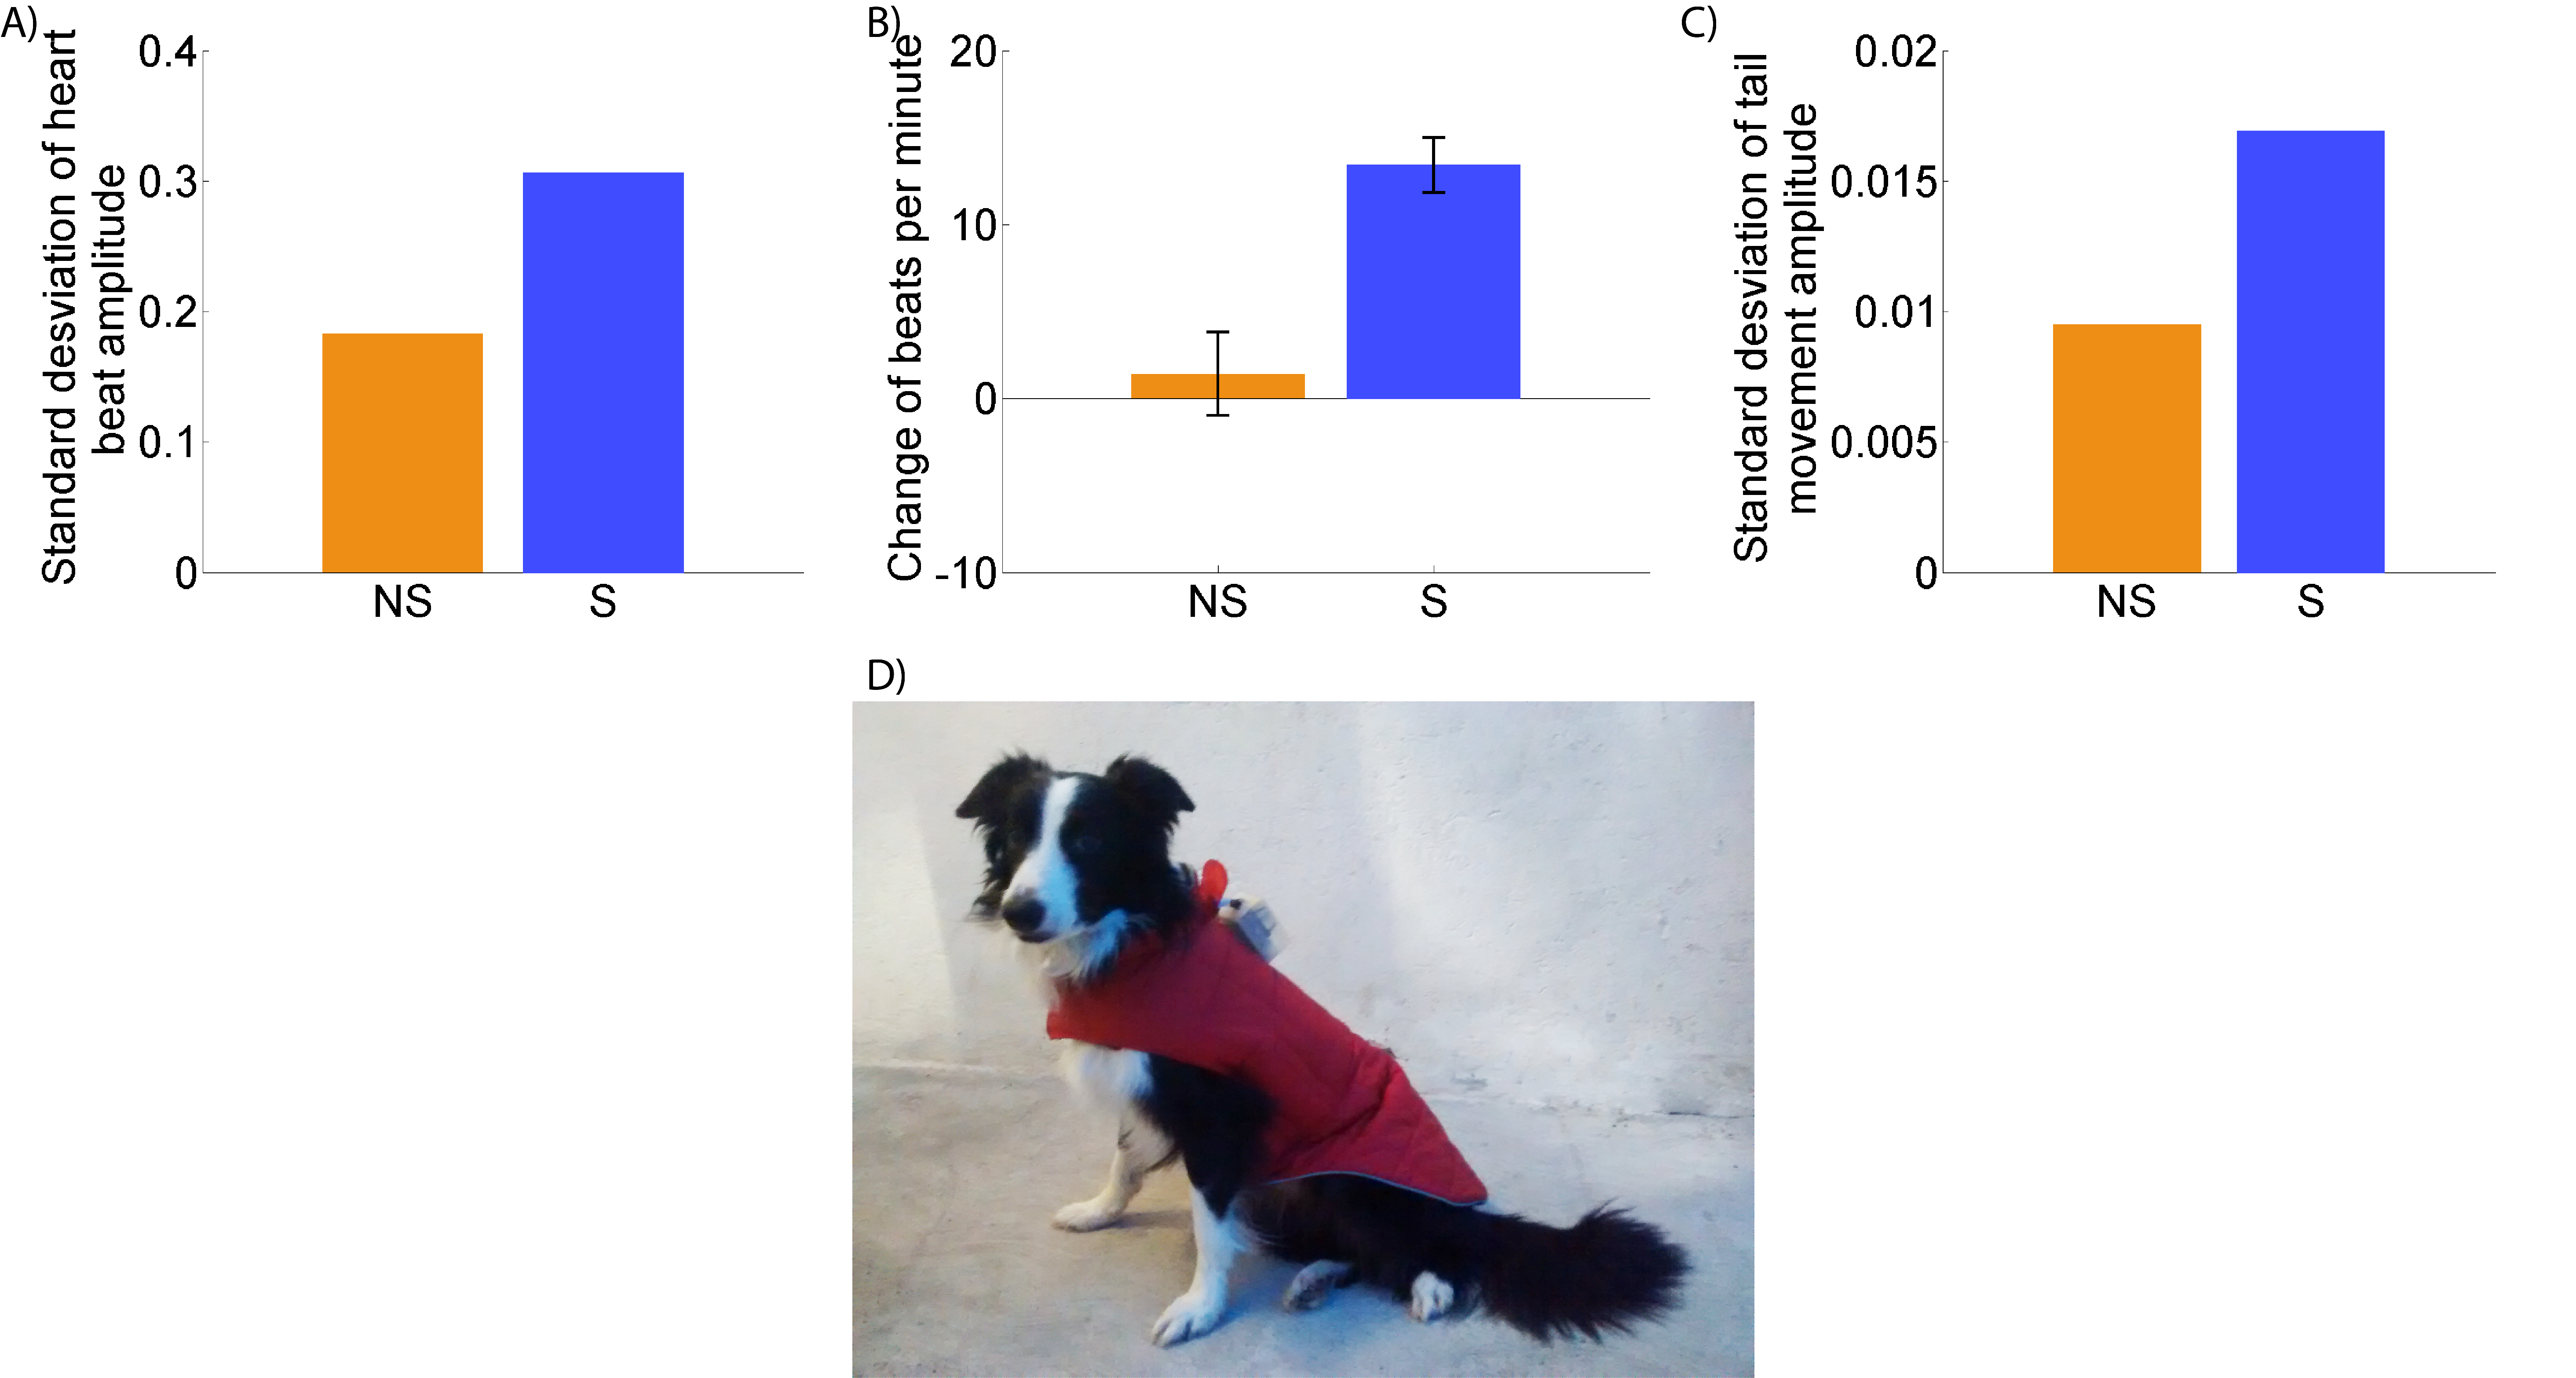
\includegraphics[width=.47\textwidth]{figure1}
  \caption{\label{centfig}
The results shown were obtained from two dogs under two consecutive conditions. Stimulation(S) and No-stimulation(NS). In panels A), B) and C), the colors represent the conditions. The panel A) represents the standard deviation from the mean of the heart beat amplitude. The panel B) represents the change on the beats per minute on both conditions minus a baseline registered directly from each dog. The vertical lines represent the standard error. The panel C) represents the standard deviation from the mean of the tail movement. The panel D) shows one of the registered dogs wearing the device.
}
\end{figure}

By matching the data collected with observations of the movement of the
tail, we notice that the data reflects the position of the tail but its
resolution depended on the position of the electrode.

The data acquired from the free movement condition was affected by the
movement and didn't seem reliable for testing.

\section{Conclusions}\label{conclusions}

We were able to build and test a non-invasive low cost device with the
capacity to register the heart rate and the tail movement of dogs. We
consider that the addition of a movement sensor could provide additional
data to reduce the change on the signal due to movement.

Even though the vibration sensor gave us adequate readings on the heart
rate in the stimulation and no stimulation conditions, the free movement
condition produced to much noise on the sensor, which results in a
limiting in the use of the device during movement, it is possible to use
different sensors such as an EKG sensor for humans that doesn't rely on
movement. In the case of the EMG sensor, both, the vibration sensor and
the EMG sensor can be replaced or new sensors can be added.

This device can be integrated in future research on dog's cognition. It
can also be used in shelters and homes to easily measure the responses
that dogs present to different sets of stimuli; for example, when a dog
is left alone in its house and shows stress (i.e.~increased heart rate,
preferential tail movement to the left) the dog's carer could make
changes in the environment to increase the well-being of the dog.

The low cost and the easy access to the materials needed to build the
device make it a feasible option to study dog cognition.

%%%%%%%%%%%%%%%%%%%%%%%%%%%%%%%%%%%%%%%%%%%%%%
%%                                          %%
%% Backmatter begins here                   %%
%%                                          %%
%%%%%%%%%%%%%%%%%%%%%%%%%%%%%%%%%%%%%%%%%%%%%%

\begin{backmatter}

\section*{Availability of Supporting Data}
More information about this project can be found at: \url{https://github.com/nekrum/DogVest}. Further data and files supporting this project are hosted in the \emph{GigaScience} repository REFXXX.

\section*{Competing interests}
None

\section*{Author's contributions}
LVC generated the idea for the project, made the research, help writing
the report and acquire the data. EAM and RH designed the device, build
it, wrote the code and help writing the report.

\section*{Acknowledgements}
We would like to thank the organizers and attendees of Brainhack MX and
to the Instituto de Neurobiología. Specially to Fernando Barrios Alvarez
for the invitation and the support on the realization of the project.
Laura V. Cuaya, Raul Hernández and Edgar Morales are a doctoral students
from Programa de Doctorado en Ciencias Biomédicas, Universidad Nacional
Autónoma de México (UNAM) and received fellowship 407590, 409258 and
215702 from CONACYT.

  
  
%%%%%%%%%%%%%%%%%%%%%%%%%%%%%%%%%%%%%%%%%%%%%%%%%%%%%%%%%%%%%
%%                  The Bibliography                       %%
%%                                                         %%
%%  Bmc_mathpys.bst  will be used to                       %%
%%  create a .BBL file for submission.                     %%
%%  After submission of the .TEX file,                     %%
%%  you will be prompted to submit your .BBL file.         %%
%%                                                         %%
%%                                                         %%
%%  Note that the displayed Bibliography will not          %%
%%  necessarily be rendered by Latex exactly as specified  %%
%%  in the online Instructions for Authors.                %%
%%                                                         %%
%%%%%%%%%%%%%%%%%%%%%%%%%%%%%%%%%%%%%%%%%%%%%%%%%%%%%%%%%%%%%

% if your bibliography is in bibtex format, use those commands:
\bibliographystyle{bmc-mathphys} % Style BST file
\bibliography{brainhack-report} % Bibliography file (usually '*.bib' )

\end{backmatter}
\end{document}
